\documentclass{article}
\usepackage{fancyhdr}
\usepackage{ctex}
\usepackage{listings}
\usepackage{graphicx}
\usepackage[a4paper, body={18cm,22cm}]{geometry}
\usepackage{amsmath,amssymb,amstext,wasysym,enumerate,graphicx}
\usepackage{float,abstract,booktabs,indentfirst,amsmath}
\usepackage{array}
\usepackage{booktabs}
\usepackage{multirow}
\usepackage{url}
\usepackage{diagbox}
\renewcommand\arraystretch{1.4}
\usepackage{indentfirst}
\setlength{\parindent}{2em}
\usepackage{enumitem}
\setmonofont{JetBrains Mono}
\usepackage{listings}
\usepackage{xcolor}
\usepackage{makecell}
\usepackage{tikz}
\usetikzlibrary{positioning, arrows.meta}
\setCJKmonofont{黑体}
\lstset{
    % language = C,
    xleftmargin = 3em,xrightmargin = 3em, aboveskip = 1em,
	backgroundcolor = \color{white}, % 背景色
	basicstyle = \small\ttfamily, % 基本样式 + 小号字体
	rulesepcolor= \color{gray}, % 代码块边框颜色
	breaklines = true, % 代码过长则换行
	numbers = left, % 行号在左侧显示
	numberstyle = \small, % 行号字体
    numbersep = -14pt, 
    keywordstyle=\color{purple}\bfseries, % 关键字颜色
    commentstyle =\color{red!50!green!50!blue!60}, % 注释颜色
    stringstyle = \color{red!60!green!90!blue!90}, % 字符串颜色
    morekeywords={ASSERT, int64_t, uint32_t},
	frame = shadowbox, % 用(带影子效果)方框框住代码块
	showspaces = false, % 不显示空格
	columns = fixed, % 字间距固定
} 
\lstset{
    sensitive=true,
    moreemph={ASSERT, NULL}, emphstyle=\color{red}\bfseries,
    moreemph=[2]{int64_t, uint32_t, tid_t, uint8_t, int16_t, uint16_t, int32_t, size_t, bool}, emphstyle=[2]\color{purple}\bfseries,
    commentstyle=\color{green!60!black}, % 设置注释颜色
    morecomment=[l][\color{green!60!black}]{+}, % 设置以+开头的代码行为绿色
}
%--------------------页眉--------------------%
\pagestyle{fancy}
\fancyhead[L]{}
\fancyhead[R]{}
\fancyhead[C]{华东师范大学软件工程学院实验报告}
\fancyfoot[C]{-\thepage-}
\renewcommand{\headrulewidth}{1.5pt}
%--------------------标题--------------------%
\begin{document}
\begin{center}
  {\Large{\textbf{\heiti 华东师范大学软件工程学院实验报告}}}
  \begin{table}[H]
    \centering
    \begin{tabular}{p{2cm}p{4cm}<{\centering}p{1cm}p{2cm}p{6cm}<{\centering}}
      姓\qquad 名: & 李鹏达    & \quad & 学\qquad 号: & 10225101460         \\ \cline{2-2} \cline{5-5}
      实验编号:    & Project 1 & \quad & 实验名称:    & {Threads in Pintos}
      \\ \cline{2-2} \cline{5-5}
    \end{tabular}
  \end{table}
\end{center}
\rule{\textwidth}{1pt}
%--------------------正文--------------------%
\section{实验目的}

\begin{enumerate}[noitemsep, label={{\arabic*})}]
  \item 重新实现 \texttt{timer\_sleep()}函数,以避免进程在就绪和运行状态间的不停切换
  \item 实现优先级调度
  \item 实现多级反馈调度
\end{enumerate}
\normalsize
\section{实验内容与实验步骤}
在本实验中,我们将对原有的进程调度功能进行三部分的改进:

\begin{enumerate}[noitemsep, label={{\arabic*})}]
  \item 重新实现\texttt{timer\_sleep()}函数,以避免进程在就绪和运行状态间的不停切换。
  \item 实现优先级调度
  \item 实现多级反馈调度
\end{enumerate}

最终达到目标——使该项目的27个检测点全部通过。


主要探讨了时钟、进程状态、优先级调度(抢占)、信号量这四大问题。


\subsection{重新实现\texttt{timer\_sleep()}函数}
首先我们先查看原本的\texttt{timer\_sleep()}函数的实现。

\begin{lstlisting}[xleftmargin = 4em,xrightmargin = 4em, aboveskip = 1em, numbers = left, language = C,title=原本的\texttt{timer\_sleep()}函数]
    /* Sleeps for approximately TICKS timer ticks.  Interrupts must
   be turned on. */
    void
    timer_sleep (int64_t ticks) 
    {
    int64_t start = timer_ticks ();

    ASSERT (intr_get_level () == INTR_ON);
    while (timer_elapsed (start) < ticks) 
        thread_yield ();
    }
\end{lstlisting}

可以发现,它的实现是通过查询当前等待时间是否小于应等待时间,如果小于应等待时间,则不断的调用\texttt{thread\_yield()}函数来实现的。

接下来,我们查看\texttt{thread\_yield()}函数的实现。

\begin{lstlisting}[xleftmargin = 4em,xrightmargin = 4em, aboveskip = 1em, numbers = left, language = C,title=原本的\texttt{thread\_yield()}函数]
    /* Yields the CPU.  The current thread is not put to sleep and
   may be scheduled again immediately at the scheduler's whim. */
    void
    thread_yield (void) 
    {
    struct thread *cur = thread_current ();
    enum intr_level old_level;

    ASSERT (!intr_context ());

    old_level = intr_disable ();
    if (cur != idle_thread) 
        list_push_back (&ready_list, &cur->elem);
    cur->status = THREAD_READY;
    schedule ();
    intr_set_level (old_level);
    }
\end{lstlisting}

可以发现,\texttt{thread\_yield()}函数的实现,是不断检查当前线程是否为空闲线程,如果不是,则将当前线程放置到就绪队列的末尾,然后将当前线程的状态设置为\texttt{THREAD\_READY},最后调用\texttt{schedule()}函数来进行调度。

这样的实现方式,会导致线程在就绪和运行状态间的不停切换,从而导致CPU资源的浪费。所以我们需要重新实现\texttt{timer\_sleep()}函数,使得线程在休眠的时候不会占用CPU资源。

可以考虑在线程结构体中增加一个成员变量\texttt{int64\_t sleep\_ticks},用来记录线程应该休眠的时间。

\begin{lstlisting}[xleftmargin = 4em,xrightmargin = 4em, aboveskip = 1em, numbers = left, language = C, title=修改后的线程结构体]
    struct thread
      {
        /* Owned by thread.c. */
        tid_t tid;                          /* Thread identifier. */
        enum thread_status status;          /* Thread state. */
        char name[16];                      /* Name (for debugging purposes). */
        uint8_t *stack;                     /* Saved stack pointer. */
        int priority;                       /* Priority. */
        struct list_elem allelem;           /* List element for all threads list. */

        /* Shared between thread.c and synch.c. */
        struct list_elem elem;              /* List element. */

        /* 应该休眠的时间 */
        int64_t sleep_ticks;                /* Sleep ticks. */

    #ifdef USERPROG
        /* Owned by userprog/process.c. */
        uint32_t *pagedir;                  /* Page directory. */
    #endif

        /* Owned by thread.c. */
        unsigned magic;                     /* Detects stack overflow. */
      };
\end{lstlisting}

接下来,我们需要初始化这个成员变量,我们在\texttt{thread\_create()}函数中,将\texttt{sleep\_ticks}初始化为0。

\begin{lstlisting}[xleftmargin = 4em,xrightmargin = 4em, aboveskip = 1em, numbers = left, language = C, title=修改后的\texttt{thread\_create()}函数]
    tid_t
    thread_create (const char *name, int priority,
                  thread_func *function, void *aux) 
    {
      struct thread *t;
      struct kernel_thread_frame *kf;
      struct switch_entry_frame *ef;
      struct switch_threads_frame *sf;
      tid_t tid;
    
      ASSERT (function != NULL);
    
      /* Allocate thread. */
      t = palloc_get_page (PAL_ZERO);
      if (t == NULL)
        return TID_ERROR;
    
      /* Initialize thread. */
      init_thread (t, name, priority);
      tid = t->tid = allocate_tid ();
      t->sleep_ticks = 0; // 初始化 sleep_ticks 为 0
    
      /* Stack frame for kernel_thread(). */
      kf = alloc_frame (t, sizeof *kf);
      kf->eip = NULL;
      kf->function = function;
      kf->aux = aux;
    
      /* Stack frame for switch_entry(). */
      ef = alloc_frame (t, sizeof *ef);
      ef->eip = (void (*) (void)) kernel_thread;
    
      /* Stack frame for switch_threads(). */
      sf = alloc_frame (t, sizeof *sf);
      sf->eip = switch_entry;
      sf->ebp = 0;
    
      /* Add to run queue. */
      thread_unblock (t);
    
      return tid;
    }
\end{lstlisting}


接下来在\texttt{timer\_sleep()}函数中,将当前线程的\texttt{sleep\_ticks}设置为应该等待的时间,接着,我们调用\texttt{thread\_block()}函数将当前线程阻塞。注意,我们需要先关闭中断,防止在设置\texttt{sleep\_ticks}和阻塞线程的过程中,被其他线程抢占,从而导致\texttt{sleep\_ticks}被修改,或者线程被重新加入就绪队列。需要注意的是,如果休眠时间小于等于0,则直接返回。

\begin{lstlisting}[xleftmargin = 4em,xrightmargin = 4em, aboveskip = 1em, numbers = left, language = C, title=修改后的\texttt{timer\_sleep()}函数]
    /* Sleeps for approximately TICKS timer ticks.  Interrupts must
      be turned on. */
    void
    timer_sleep (int64_t ticks) 
    {
      if (ticks <= 0) // 如果休眠时间小于等于 0
      {
        return; // 直接返回
      }

      ASSERT (intr_get_level () == INTR_ON);
      
      enum intr_level old_level = intr_disable (); // 关闭中断
      thread_current ()->sleep_ticks = ticks; // 设置 sleep_ticks
      thread_block (); // 阻塞当前线程
      INTR_set_level (old_level); // 恢复中断
    }
\end{lstlisting}

接下来,我们需要修改\texttt{timmer\_interrupt()}函数,来实现对\texttt{sleep\_ticks}的更新。首先,我们需要遍历所有线程,将\texttt{sleep\_ticks}减一,如果\texttt{sleep\_ticks}为0,则将线程唤醒。为了遍历线程,我们需要使用\texttt{thread\_foreach()}函数,它可以对每个线程调用一个函数,我们需要编写这个函数来实现对\texttt{sleep\_ticks}的更新。

\begin{lstlisting}[xleftmargin = 4em,xrightmargin = 3em, aboveskip = 1em, numbers = left, language = C, title=修改后的\texttt{timmer\_interrupt()}函数]
    /* Timer interrupt handler. */
    static void
    timer_interrupt (struct intr_frame *args UNUSED)
    {
      ticks++;
      thread_tick ();
      thread_foreach (thread_tick_sleep, NULL); // 每次中断都调用 
    }
    
    /* 休眠时间到了就唤醒 */
    void
    thread_tick_sleep (struct thread *t, void *aux UNUSED)
    {
      if (t->status == THREAD_BLOCKED && t->sleep_ticks > 0) // 如果休眠时间大于 0
      {
        t->sleep_ticks--; // 休眠时间减一
        if (t->sleep_ticks == 0) // 如果休眠时间到了
        {
          thread_unblock (t); // 唤醒
        }
      }
    }
\end{lstlisting}

这样,我们就完成了对\texttt{timer\_sleep()}函数的重新实现。

\subsection{实现优先级调度}

\subsubsection{测试\texttt{alarm-priority, priority-change, priority-fifo}和\texttt{priority-preempt}}


在原本的实现中,线程的调度是按照FIFO的顺序进行的,这样会导致优先级高的线程无法优先执行。所以我们需要实现优先级调度,使得优先级高的线程能够优先执行。

由于在pintos中有一个已经定义好的按顺序插入的函数\texttt{list\_insert\_ordered()},所以我们可以使用这个函数来实现优先级调度。\texttt{list\_insert\_ordered()}函数的定义如下:

\begin{lstlisting}[xleftmargin = 4em,xrightmargin = 3em, aboveskip = 1em, numbers = left, language = C, title=\texttt{list\_insert\_ordered()}函数的定义]
    /* Inserts ELEM in the list in sorted order. */
    void
    list_insert_ordered (struct list *list, struct list_elem *elem,
                         list_less_func *less_func, void *aux)
    {
      struct list_elem *e;
    
      ASSERT (list != NULL);
      ASSERT (elem != NULL);
      ASSERT (less_func != NULL);
    
      for (e = list_begin (list); e != list_end (list); e = list_next (e))
        if (less_func (elem, e, aux))
          break;
      list_insert (e, elem);
    }

\end{lstlisting}


首先,我们需要实现一个比较函数,用来比较两个线程的优先级。

\begin{lstlisting}[xleftmargin = 4em,xrightmargin = 3em, aboveskip = 1em, numbers = left, language = C, title=比较函数]
    /* 比较函数 */
    bool
    thread_priority_cmp (const struct list_elem *a, const struct list_elem *b, void *aux UNUSED)
    {
      struct thread *ta = list_entry (a, struct thread, elem);
      struct thread *tb = list_entry (b, struct thread, elem);
      return ta->priority > tb->priority;
    }

\end{lstlisting}

然后,我们需要修改\texttt{thread\_unblock()},\texttt{thread\_yield()}和\texttt{thread\_init()}这三个函数,使得线程在被唤醒、主动让出CPU和初始化的时候,按照优先级的顺序插入就绪队列。

\begin{lstlisting}[xleftmargin = 4em,xrightmargin = 3em, aboveskip = 1em, numbers = left, language = C, title=对相关函数的修改]
    void
    thread_unblock (struct thread *t) 
    {
      enum intr_level old_level;

      ASSERT (is_thread (t));

      old_level = intr_disable ();
      ASSERT (t->status == THREAD_BLOCKED);
      list_insert_ordered (&ready_list, &t->elem, thread_priority_cmp, NULL); // 按优先级排序
      t->status = THREAD_READY;
      intr_set_level (old_level);
    }

    void
    thread_yield (void) 
    {
      struct thread *cur = thread_current ();
      enum intr_level old_level;
      
      ASSERT (!intr_context ());

      old_level = intr_disable ();
      if (cur != idle_thread) 
        list_insert_ordered (&ready_list, &cur->elem, thread_priority_cmp, NULL); // 按优先级排序
      cur->status = THREAD_READY;
      schedule ();
      intr_set_level (old_level);
    }

    static void
    init_thread (struct thread *t, const char *name, int priority)
    {
      enum intr_level old_level;

      ASSERT (t != NULL);
      ASSERT (PRI_MIN <= priority && priority <= PRI_MAX);
      ASSERT (name != NULL);

      memset (t, 0, sizeof *t);
      t->status = THREAD_BLOCKED;
      strlcpy (t->name, name, sizeof t->name);
      t->stack = (uint8_t *) t + PGSIZE;
      t->priority = priority;
      t->magic = THREAD_MAGIC;

      old_level = intr_disable ();
      list_insert_ordered (&all_list, &t->allelem, thread_priority_cmp, NULL); // 按优先级排序
      intr_set_level (old_level);
    }
  
\end{lstlisting}


接下来,我们需要修改\texttt{thread\_create()}函数,使得线程在创建的时候,按照优先级的顺序插入就绪队列。

\begin{lstlisting}[xleftmargin = 4em,xrightmargin = 3em, aboveskip = 1em, numbers = left, language = C, title=修改后的\texttt{thread\_create()}函数]
    tid_t
    thread_create (const char *name, int priority,
                  thread_func *function, void *aux) 
    {
      struct thread *t;
      struct kernel_thread_frame *kf;
      struct switch_entry_frame *ef;
      struct switch_threads_frame *sf;
      tid_t tid;
    
      ASSERT (function != NULL);
    
      /* Allocate thread. */
      t = palloc_get_page (PAL_ZERO);
      if (t == NULL)
        return TID_ERROR;
    
      /* Initialize thread. */
      init_thread (t, name, priority);
      tid = t->tid = allocate_tid ();
      t->sleep_ticks = 0;
    
      /* Stack frame for kernel_thread(). */
      kf = alloc_frame (t, sizeof *kf);
      kf->eip = NULL;
      kf->function = function;
      kf->aux = aux;
    
      /* Stack frame for switch_entry(). */
      ef = alloc_frame (t, sizeof *ef);
      ef->eip = (void (*) (void)) kernel_thread;
    
      /* Stack frame for switch_threads(). */
      sf = alloc_frame (t, sizeof *sf);
      sf->eip = switch_entry;
      sf->ebp = 0;
    
      /* Add to run queue. */
      thread_unblock (t);
    
      /* 优先级调度 */
      if (thread_current ()->priority < priority)
      {
        thread_yield ();
      }
    
      return tid;
    }
\end{lstlisting}

然后,我们需要修改\texttt{thread\_set\_priority()}函数,使得线程在修改优先级的时候,重新调度。

\begin{lstlisting}[xleftmargin = 4em,xrightmargin = 3em, aboveskip = 1em, numbers = left, language = C, title=修改后的\texttt{thread\_set\_priority()}函数]
    void
    thread_set_priority (int new_priority) 
    {
      enum intr_level old_level = intr_disable ();
      int old_priority = thread_current ()->priority;
      thread_current ()->priority = new_priority;
      thread_yield (); // 重新调度
      intr_set_level (old_level);
    }
\end{lstlisting}

这样,我们就可以通过测试 \texttt{alarm-priority, priority-change, priority-fifo}和\\ \texttt{priority-preempt}了。

接下来,我们需要实现优先级捐赠。

我们可以先阅读测试文件,分析需要进行哪些修改。

\subsubsection{测试\texttt{priority-donate-one}}

首先,我们分析 \texttt{priority-donate-one}测试,它的代码如下:

\begin{lstlisting}[xleftmargin = 4em,xrightmargin = 3em, aboveskip = 1em, numbers = left, language = C, title=\texttt{priority-donate-one}测试]
    static thread_func acquire1_thread_func;
    static thread_func acquire2_thread_func;

    void
    test_priority_donate_one (void) 
    {
      struct lock lock;

      /* This test does not work with the MLFQS. */
      ASSERT (!thread_mlfqs);

      /* Make sure our priority is the default. */
      ASSERT (thread_get_priority () == PRI_DEFAULT);

      lock_init (&lock);
      lock_acquire (&lock);
      thread_create ("acquire1", PRI_DEFAULT + 1, acquire1_thread_func, &lock);
      msg ("This thread should have priority %d.  Actual priority: %d.",
          PRI_DEFAULT + 1, thread_get_priority ());
      thread_create ("acquire2", PRI_DEFAULT + 2, acquire2_thread_func, &lock);
      msg ("This thread should have priority %d.  Actual priority: %d.",
          PRI_DEFAULT + 2, thread_get_priority ());
      lock_release (&lock);
      msg ("acquire2, acquire1 must already have finished, in that order.");
      msg ("This should be the last line before finishing this test.");
    }

    static void
    acquire1_thread_func (void *lock_) 
    {
      struct lock *lock = lock_;

      lock_acquire (lock);
      msg ("acquire1: got the lock");
      lock_release (lock);
      msg ("acquire1: done");
    }

    static void
    acquire2_thread_func (void *lock_) 
    {
      struct lock *lock = lock_;

      lock_acquire (lock);
      msg ("acquire2: got the lock");
      lock_release (lock);
      msg ("acquire2: done");
    }

\end{lstlisting}

以下是测试的主要步骤和分析:

1. \textbf{初始化锁:}
\begin{lstlisting}[language=C]
    struct lock lock;
    lock_init(&lock);
\end{lstlisting}

在测试开始时,创建一个锁以供线程之间同步和竞争。

2. \textbf{主线程获取锁:}
\begin{lstlisting}[language=C]
    lock_acquire(&lock);    
\end{lstlisting}

主线程获取锁,此时它的优先级是默认优先级 \texttt{PRI\_DEFAULT}。

3. \textbf{创建两个高优先级的线程:}
\begin{lstlisting}[language=C]
    thread_create("acquire1", PRI_DEFAULT + 1, acquire1_thread_func, &lock);
    thread_create("acquire2", PRI_DEFAULT + 2, acquire2_thread_func, &lock);
\end{lstlisting}

创建两个新线程,分别命名为 \texttt{acquire1} 和 \texttt{acquire2},它们的优先级分别比主线程高1和2。这两个线程被设计为在获取锁时被阻塞。

4. \textbf{释放锁:}
\begin{lstlisting}[language=C]
    lock_release(&lock);
\end{lstlisting}

主线程释放锁。由于这时两个新线程的优先级高于主线程,它们会优先尝试获取锁。

5. \textbf{\texttt{acquire2} 线程先获取锁:}
\begin{lstlisting}[language=C]
    acquire2_thread_func(void *lock_) 
    {
    // ...
      lock_acquire(lock);
      msg("acquire2: got the lock");
      lock_release(lock);
    // ...
    }
\end{lstlisting}

由于 \texttt{acquire2} 的优先级更高,它首先获取了锁。

6. \textbf{\texttt{acquire1} 线程后获取锁:}
\begin{lstlisting}[language=C]
    acquire1_thread_func(void *lock_) 
    {
    // ...
      lock_acquire(lock);
      msg("acquire1: got the lock");
      lock_release(lock);
    // ...
    }
\end{lstlisting}

由于 \texttt{acquire1} 的优先级次高,它在 \texttt{acquire2} 线程之后获取了锁。

7. \textbf{测试完成:}
\begin{lstlisting}[language=C]
    msg("acquire2, acquire1 must already have finished, in that order.");
    msg("This should be the last line before finishing this test.");
\end{lstlisting}

打印测试结果,确认 \texttt{acquire2} 线程先完成,然后是 \texttt{acquire1} 线程。

总体来说,这个测试验证了线程在释放锁时是否正确地将其优先级传递给等待该锁的其他线程,从而确保线程按照它们的优先级顺序获取锁。

在这个测试中,主线程先持有锁,随后两个优先级更高、等待这个锁的线程被创建,于是这两个线程便会向主线程捐赠优先级。当主线程释放锁时,两个线程中优先级更高的线程会先获取锁,然后是优先级次高的线程。

为了通过这个测试,首先,我们需要修改 \texttt{lock\_acquire()}函数,使得线程在获取锁的时候,如果锁已经被占用,且当前线程的优先级大于锁的持有者的优先级,则将当前线程的优先级赋值给锁的持有者。

\begin{lstlisting}[language=C, title=修改后的\texttt{lock\_acquire()}函数]
    void
    lock_acquire (struct lock *lock)
    {
      ASSERT (lock != NULL);
      ASSERT (!intr_context ());
      ASSERT (!lock_held_by_current_thread (lock));
    
      if (lock->holder != NULL && lock->holder->priority < thread_current ()->priority)
      {
        lock->holder->priority = thread_current ()->priority;
      }
    
      sema_down (&lock->semaphore);
      lock->holder = thread_current ();
    }

\end{lstlisting}

然后,我们需要修改 \texttt{lock\_release()}函数,使得线程在释放锁的时候,将当前线程的优先级恢复为原来的优先级。

为此,我们需要在线程结构体中增加一个成员变量\texttt{int original\_priority},用来记录线程的原始优先级。

\begin{lstlisting}[language=C, title=修改后的线程结构体]
    struct thread
      {
        /* Owned by thread.c. */
        tid_t tid;                          /* Thread identifier. */
        enum thread_status status;          /* Thread state. */
        char name[16];                      /* Name (for debugging purposes). */
        uint8_t *stack;                     /* Saved stack pointer. */
        int priority;                       /* Priority. */
        struct list_elem allelem;           /* List element for all threads list. */
    
        /* Shared between thread.c and synch.c. */
        struct list_elem elem;              /* List element. */
    
        /* 应该休眠的时间 */
        int64_t sleep_ticks;                /* Sleep ticks. */
    
        /* 原始优先级 */
        int original_priority;              /* Original priority. */
    
    #ifdef USERPROG
        /* Owned by userprog/process.c. */
        uint32_t *pagedir;                  /* Page directory. */
    #endif
    
        /* Owned by thread.c. */
        unsigned magic;                     /* Detects stack overflow. */
      };

\end{lstlisting}

接下来,我们需要修改 \texttt{init\_thread()}函数,使得线程在创建的时候,将线程的原始优先级设置为线程的优先级。

\begin{lstlisting}[language=C, title=修改后的\texttt{init\_thread()}函数]
    static void
    init_thread (struct thread *t, const char *name, int priority)
    {
      enum intr_level old_level;

      ASSERT (t != NULL);
      ASSERT (PRI_MIN <= priority && priority <= PRI_MAX);
      ASSERT (name != NULL);

      memset (t, 0, sizeof *t);
      t->status = THREAD_BLOCKED;
      strlcpy (t->name, name, sizeof t->name);
      t->stack = (uint8_t *) t + PGSIZE;
      t->priority = priority;
      t->original_priority = priority;
      t->magic = THREAD_MAGIC;

      old_level = intr_disable ();
      list_insert_ordered (&all_list, &t->allelem, thread_priority_cmp, NULL);
      intr_set_level (old_level);
    }

\end{lstlisting}

然后,我们修改 \texttt{lock\_release()}函数,使得线程在释放锁的时候,将当前线程的优先级恢复为原来的优先级。

\begin{lstlisting}[language=C, title=修改后的\texttt{lock\_release()}函数]
    void
    lock_release (struct lock *lock) 
    {
      ASSERT (lock != NULL);
      ASSERT (lock_held_by_current_thread (lock));
    
      lock->holder = NULL;
      sema_up (&lock->semaphore);
      
      thread_set_priority (thread_current ()->original_priority);
    }

\end{lstlisting}

最后,我们修改 \texttt{sema\_down} 函数,保证等待锁的线程按照优先级顺序排列。

\begin{lstlisting}[language=C, title=修改后的\texttt{sema\_down()}函数]
    void
    sema_down (struct semaphore *sema) 
    {
      enum intr_level old_level;
    
      ASSERT (sema != NULL);
      ASSERT (!intr_context ());
    
      old_level = intr_disable ();
      while (sema->value == 0) 
        {
          list_insert_ordered (&sema->waiters, &thread_current ()->elem, thread_priority_cmp, NULL);
          thread_block ();
        }
      sema->value--;
      intr_set_level (old_level);
    }
\end{lstlisting}

这样,我们就可以通过测试 \texttt{priority-donate-one}了。

\subsubsection{测试\texttt{priority-donate-multiple}和 \texttt{priority-donate-multiple2}}

接下来,我们分析 \texttt{priority-donate-multiple2}测试,它的代码如下:

\begin{lstlisting}[language=C, title=\texttt{priority-donate-multiple2}测试]
    static thread_func a_thread_func;
    static thread_func b_thread_func;
    static thread_func c_thread_func;

    void
    test_priority_donate_multiple2 (void) 
    {
      struct lock a, b;

      /* This test does not work with the MLFQS. */
      ASSERT (!thread_mlfqs);

      /* Make sure our priority is the default. */
      ASSERT (thread_get_priority () == PRI_DEFAULT);

      lock_init (&a);
      lock_init (&b);

      lock_acquire (&a);
      lock_acquire (&b);

      thread_create ("a", PRI_DEFAULT + 3, a_thread_func, &a);
      msg ("Main thread should have priority %d.  Actual priority: %d.",
            PRI_DEFAULT + 3, thread_get_priority ());

      thread_create ("c", PRI_DEFAULT + 1, c_thread_func, NULL);

      thread_create ("b", PRI_DEFAULT + 5, b_thread_func, &b);
      msg ("Main thread should have priority %d.  Actual priority: %d.",
            PRI_DEFAULT + 5, thread_get_priority ());

      lock_release (&a);
      msg ("Main thread should have priority %d.  Actual priority: %d.",
            PRI_DEFAULT + 5, thread_get_priority ());

      lock_release (&b);
      msg ("Threads b, a, c should have just finished, in that order.");
      msg ("Main thread should have priority %d.  Actual priority: %d.",
            PRI_DEFAULT, thread_get_priority ());
    }

    static void
    a_thread_func (void *lock_) 
    {
      struct lock *lock = lock_;

      lock_acquire (lock);
      msg ("Thread a acquired lock a.");
      lock_release (lock);
      msg ("Thread a finished.");
    }

    static void
    b_thread_func (void *lock_) 
    {
      struct lock *lock = lock_;

      lock_acquire (lock);
      msg ("Thread b acquired lock b.");
      lock_release (lock);
      msg ("Thread b finished.");
    }

    static void
    c_thread_func (void *a_ UNUSED) 
    {
      msg ("Thread c finished.");
    }

\end{lstlisting}

以下是对测试步骤的分析:

1. \textbf{初始化锁:}
\begin{lstlisting}[language=C]
    struct lock a, b;
    lock_init(&a);
    lock_init(&b);
\end{lstlisting}

在测试开始时,创建两个锁,命名为 \texttt{a} 和 \texttt{b},用于线程之间的同步。

2. \textbf{主线程获取锁 \texttt{a} 和 \texttt{b}:}
\begin{lstlisting}[language=C]
    lock_acquire(&a);
    lock_acquire(&b);
\end{lstlisting}

主线程获取两个锁 \texttt{a} 和 \texttt{b}。

3. \textbf{创建三个高优先级的线程:}
\begin{lstlisting}[language=C]
    thread_create("a", PRI_DEFAULT + 3, a_thread_func, &a);
    thread_create("c", PRI_DEFAULT + 1, c_thread_func, NULL);
    thread_create("b", PRI_DEFAULT + 5, b_thread_func, &b);
\end{lstlisting}

创建三个新线程,分别命名为 \texttt{a}、\texttt{c} 和 \texttt{b},它们的优先级分别比主线程高3、1和5。

4. \textbf{释放锁 \texttt{a} 和 \texttt{b}:}
\begin{lstlisting}[language=C]
    lock_release(&a);
    lock_release(&b);
\end{lstlisting}

主线程释放两个锁。

5. \textbf{测试结果输出:}
\begin{lstlisting}[language=C]
    msg ("Main thread should have priority %d.  Actual priority: %d.",
    PRI_DEFAULT + 3, thread_get_priority ());
    // ...
    msg ("Main thread should have priority %d.  Actual priority: %d.",
    PRI_DEFAULT + 5, thread_get_priority ());
    // ...
    msg ("Main thread should have priority %d.  Actual priority: %d.",
    PRI_DEFAULT + 5, thread_get_priority ());
    // ...
    msg("Threads b, a, c should have just finished, in that order.");
    msg("Main thread should have priority %d.  Actual priority: %d.",
        PRI_DEFAULT, thread_get_priority ());
\end{lstlisting}

打印测试结果,确认主线程拥有正确的优先级,且最后线程 \texttt{b}、\texttt{a}、\texttt{c} 已经完成,按照优先级的顺序。

总体来说,这个测试验证了在有多个锁的情况下,线程在释放锁时,是否正确地将其优先级设为剩余锁的最高优先级,从而确保线程按照它们的优先级顺序获取锁。

为了通过这个测试,首先,我们必须记录线程持有的锁,为此,我们需要在线程结构体中增加一个成员变量\texttt{struct list locks},用来记录线程持有的锁。

\begin{lstlisting}[language=C, title=修改后的线程结构体]
      struct thread
      {
        /* Owned by thread.c. */
        tid_t tid;                          /* Thread identifier. */
        enum thread_status status;          /* Thread state. */
        char name[16];                      /* Name (for debugging purposes). */
        uint8_t *stack;                     /* Saved stack pointer. */
        int priority;                       /* Priority. */
        struct list_elem allelem;           /* List element for all threads list. */

        /* Shared between thread.c and synch.c. */
        struct list_elem elem;              /* List element. */

        /* 应该休眠的时间 */
        int64_t sleep_ticks;

        /* 原本的优先级 */
        int original_priority;               /* Orignal Priority*/

        /* 线程的锁 */
        struct list locks;                   /* Locks that the thread is holding */

    #ifdef USERPROG
        /* Owned by userprog/process.c. */
        uint32_t *pagedir;                  /* Page directory. */
    #endif

        /* Owned by thread.c. */
        unsigned magic;                     /* Detects stack overflow. */
      };

\end{lstlisting}

同时,我们还必须记录想要获取这个锁的线程的最高优先级,为此,我们需要在锁结构体中增加成员变量\texttt{int max\_priority}和 \texttt{struct list\_elem elem},用来记录想要获取这个锁的线程的最高优先级和用于插入列表的变量。

\begin{lstlisting}[language=C, title=修改后的锁结构体]
    struct lock 
    {
      struct thread *holder;      /* Thread holding lock (for debugging). */
      struct semaphore semaphore; /* Binary semaphore controlling access. */
      int max_priority;           /* Maximum priority of threads waiting for lock. */
      struct list_elem elem;      /* List element for priority donation. */
    };
\end{lstlisting}

然后,我们修改 \texttt{lock\_init()}函数,使得线程在初始化锁的时候,将锁的最高优先级初始化为 \texttt{PRI\_MIN}。

\begin{lstlisting}[language=C, title=修改后的\texttt{lock\_init()}函数]
    void
    lock_init (struct lock *lock)
    {
      ASSERT (lock != NULL);

      lock->holder = NULL;
      lock->max_priority = PRI_MIN; // 初始化为 PRI_MIN
      sema_init (&lock->semaphore, 1);
    }

\end{lstlisting}

接下来,我们修改线程结构体,添加成员变量\texttt{struct list locks},用来记录线程持有的锁。

\begin{lstlisting}[language=C, title=修改后的线程结构体]
      struct thread
      {
        /* Owned by thread.c. */
        tid_t tid;                          /* Thread identifier. */
        enum thread_status status;          /* Thread state. */
        char name[16];                      /* Name (for debugging purposes). */
        uint8_t *stack;                     /* Saved stack pointer. */
        int priority;                       /* Priority. */
        struct list_elem allelem;           /* List element for all threads list. */

        /* Shared between thread.c and synch.c. */
        struct list_elem elem;              /* List element. */

        /* 应该休眠的时间 */
        int64_t sleep_ticks;

        /* 原本的优先级 */
        int original_priority;              /* Orignal Priority*/

        /* 持有的锁 */
        struct list locks;                  /* List of locks that the thread is holding. */

    #ifdef USERPROG
        /* Owned by userprog/process.c. */
        uint32_t *pagedir;                  /* Page directory. */
    #endif

        /* Owned by thread.c. */
        unsigned magic;                     /* Detects stack overflow. */
      };
\end{lstlisting}

然后,我们修改 \texttt{init\_thread()}函数,使得线程在创建的时,初始化线程持有的锁列表。

\begin{lstlisting}[language=C, title=修改后的\texttt{init\_thread()}函数]
    static void
    init_thread (struct thread *t, const char *name, int priority)
    {
      enum intr_level old_level;

      ASSERT (t != NULL);
      ASSERT (PRI_MIN <= priority && priority <= PRI_MAX);
      ASSERT (name != NULL);

      memset (t, 0, sizeof *t);
      t->status = THREAD_BLOCKED;
      strlcpy (t->name, name, sizeof t->name);
      t->stack = (uint8_t *) t + PGSIZE;
      t->priority = priority;
      t->original_priority = priority;
      t->magic = THREAD_MAGIC;

      list_init (&t->locks); // 初始化锁列表

      old_level = intr_disable ();
      list_insert_ordered (&all_list, &t->allelem, thread_priority_cmp, NULL);
      intr_set_level (old_level);
    }

\end{lstlisting}

然后,我们实现一个锁的比较函数,用来比较两个锁的最高优先级。

\begin{lstlisting}[language=C, title=锁的比较函数]
    bool
    lock_priority_cmp (const struct list_elem *a, const struct list_elem *b, void *aux UNUSED)
    {
      struct lock *la = list_entry (a, struct lock, elem);
      struct lock *lb = list_entry (b, struct lock, elem);
      return la->max_priority > lb->max_priority;
    }

\end{lstlisting}

接下来,我们修改 \texttt{lock\_acquire()}函数,使得线程在获取锁的时候,如果锁已经被占用,且当前线程的优先级大于锁的持有者的优先级,则将当前线程的优先级赋值给锁的持有者,并将锁加入线程持有的锁列表中,并更新锁的最高优先级。

\begin{lstlisting}[language=C, title=修改后的\texttt{lock\_acquire()}函数]
    void
    lock_acquire (struct lock *lock)
    {
      ASSERT (lock != NULL);
      ASSERT (!intr_context ());
      ASSERT (!lock_held_by_current_thread (lock));
    
      if (lock->holder != NULL && lock->holder->priority < thread_current ()->priority)
      {
        lock->holder->priority = thread_current ()->priority;
        if (lock->max_priority < thread_current ()->priority)
          lock->max_priority = thread_current ()->priority;
      }
    
      sema_down (&lock->semaphore);
    
      list_insert_ordered (&thread_current ()->locks, &lock->elem, lock_priority_cmp, NULL);
      lock->holder = thread_current ();
    }

\end{lstlisting}

最后,我们修改 \texttt{lock\_release()}函数,使得线程在释放锁的时候,将当前线程的优先级恢复(如果不持有锁,则恢复为初始优先级;若持有锁,则设置为所持有锁的最高优先级)。

\begin{lstlisting}[language=C, title=修改后的\texttt{lock\_release()}函数]
    void
    lock_release (struct lock *lock) 
    {
      int max_priority;
    
      ASSERT (lock != NULL);
      ASSERT (lock_held_by_current_thread (lock));
    
      list_remove (&lock->elem);
      max_priority = thread_current ()->original_priority;
      if (!list_empty (&thread_current ()->locks))
      {
        list_sort (&thread_current ()->locks, lock_priority_cmp, NULL);
        struct lock *l = list_entry (list_front (&thread_current ()->locks), struct lock, elem);
        if (l->max_priority > max_priority)
          max_priority = l->max_priority;
      }
    
      thread_current ()->priority = max_priority;
    
      lock->holder = NULL;
      sema_up (&lock->semaphore);
    }

\end{lstlisting}

这样,我们就可以通过测试 \texttt{priority-donate-multiple, priority-donate-multiple2}了。

\subsubsection{测试\texttt{priority-donate-nest}}

接下来,我们分析 \texttt{priority-donate-nest}测试,它的代码如下:

\begin{lstlisting}[language=C, title=\texttt{priority-donate-nest}测试]
    static thread_func medium_thread_func;
    static thread_func high_thread_func;
    
    void
    test_priority_donate_nest (void) 
    {
      struct lock a, b;
      struct locks locks;
    
      /* This test does not work with the MLFQS. */
      ASSERT (!thread_mlfqs);
    
      /* Make sure our priority is the default. */
      ASSERT (thread_get_priority () == PRI_DEFAULT);
    
      lock_init (&a);
      lock_init (&b);
    
      lock_acquire (&a);
    
      locks.a = &a;
      locks.b = &b;
      thread_create ("medium", PRI_DEFAULT + 1, medium_thread_func, &locks);
      thread_yield ();
      msg ("Low thread should have priority %d.  Actual priority: %d.",
          PRI_DEFAULT + 1, thread_get_priority ());
    
      thread_create ("high", PRI_DEFAULT + 2, high_thread_func, &b);
      thread_yield ();
      msg ("Low thread should have priority %d.  Actual priority: %d.",
          PRI_DEFAULT + 2, thread_get_priority ());
    
      lock_release (&a);
      thread_yield ();
      msg ("Medium thread should just have finished.");
      msg ("Low thread should have priority %d.  Actual priority: %d.",
          PRI_DEFAULT, thread_get_priority ());
    }
    
    static void
    medium_thread_func (void *locks_) 
    {
      struct locks *locks = locks_;
    
      lock_acquire (locks->b);
      lock_acquire (locks->a);
    
      msg ("Medium thread should have priority %d.  Actual priority: %d.",
          PRI_DEFAULT + 2, thread_get_priority ());
      msg ("Medium thread got the lock.");
    
      lock_release (locks->a);
      thread_yield ();
    
      lock_release (locks->b);
      thread_yield ();
    
      msg ("High thread should have just finished.");
      msg ("Middle thread finished.");
    }
    
    static void
    high_thread_func (void *lock_) 
    {
      struct lock *lock = lock_;
    
      lock_acquire (lock);
      msg ("High thread got the lock.");
      lock_release (lock);
      msg ("High thread finished.");
    }
\end{lstlisting}

以下是对测试步骤的分析:

1. \textbf{初始化锁:}
\begin{lstlisting}[language=C]
    struct lock a, b;
    struct locks 
    {
      struct lock *a;
      struct lock *b;
    };
    struct locks locks;

    lock_init(&a);
    lock_init(&b);
\end{lstlisting}

在测试开始时,创建两个锁,命名为 \texttt{a} 和 \texttt{b}。同时,定义一个结构 \texttt{locks} 包含指向这两个锁的指针。

2. \textbf{主线程获取锁 \texttt{a}:}
\begin{lstlisting}[language=C]
    lock_acquire(&a);
\end{lstlisting}

低优先级的主线程获取锁 \texttt{a}。

3. \textbf{创建两个新线程:}
\begin{lstlisting}[language=C]
    thread_create("medium", PRI_DEFAULT + 1, medium_thread_func, &locks);
    thread_yield();
    msg("Low thread should have priority %d.  Actual priority: %d.",
        PRI_DEFAULT + 1, thread_get_priority ());

    thread_create("high", PRI_DEFAULT + 2, high_thread_func, &b);
    thread_yield();
    msg("Low thread should have priority %d.  Actual priority: %d.",
        PRI_DEFAULT + 2, thread_get_priority ());
\end{lstlisting}

创建一个中优先级的线程 \texttt{medium} 和一个高优先级的线程 \texttt{high}。此时,线程 \texttt{medium} 尝试获取锁 \texttt{a} 和 锁\texttt{b} 并阻塞,而线程 \texttt{high} 尝试获取锁 \texttt{b}。

4. \textbf{释放锁 \texttt{a}:}
\begin{lstlisting}[language=C]
    lock_release(&a);
    thread_yield();
    msg("Medium thread should just have finished.");
    msg("Low thread should have priority %d.  Actual priority: %d.",
        PRI_DEFAULT, thread_get_priority ());
\end{lstlisting}

主线程释放锁 \texttt{a},线程 \texttt{medium} 获取了锁并执行完毕。主线程此时重新获取控制,检查其优先级。

5. \textbf{\texttt{medium} 线程执行:}
\begin{lstlisting}[language=C]
    static void medium_thread_func(void *locks_) 
    {
      struct locks *locks = locks_;

      lock_acquire(locks->b);
      lock_acquire(locks->a);

      msg("Medium thread should have priority %d.  Actual priority: %d.",
          PRI_DEFAULT + 2, thread_get_priority ());
      msg("Medium thread got the lock.");

      lock_release(locks->a);
      thread_yield();

      lock_release(locks->b);
      thread_yield();

      msg("High thread should have just finished.");
      msg("Middle thread finished.");
    }
\end{lstlisting}

线程 \texttt{medium} 获取锁 \texttt{b},然后获取锁 \texttt{a}。由于线程 \texttt{high} 阻塞在锁 \texttt{b} 上,线程 \texttt{high} 的优先级捐赠给了线程 \texttt{medium}。线程 \texttt{medium} 执行完毕,释放锁 \texttt{a} 和 \texttt{b}。

6. \textbf{\texttt{high} 线程执行:}
\begin{lstlisting}[language=C]
    static void high_thread_func(void *lock_) 
    {
      struct lock *lock = lock_;

      lock_acquire(lock);
      msg("High thread got the lock.");
      lock_release(lock);
      msg("High thread finished.");
    }
\end{lstlisting}

线程 \texttt{high} 获取锁 \texttt{b},执行完毕后释放锁。

总体来说,这个测试验证了在不同优先级的线程之间进行嵌套优先级捐赠的情况。

可以作出如下关系图:

\begin{figure}[H]
  \centering
  \begin{tikzpicture}[>=Stealth, node distance=2cm]
    % Nodes
    \node (low) {低优先级线程 (31)};
    \node[right=of low] (medium) {中优先级线程 (32)};
    \node[right=of medium] (high) {高优先级线程 (33)};

    % Arrows
    \draw[->] (low.east) -- (medium.west) node[midway, above] {锁 \texttt{a}};
    \draw[->] (medium.east) -- (high.west) node[midway, above] {锁 \texttt{b}};

    % Priority Donations
    \draw[->, dashed] (high.south) -- ++(0, -0.5) -| (medium.south) node[midway, below] {优先级捐赠};
    \draw[->, dashed] (medium.south) -- ++(0, -0.5) -| (low.south) node[midway, below] {优先级捐赠};
  \end{tikzpicture}
  \caption{线程关系图}
\end{figure}

通过分析,我们可以得知,优先级捐赠需要递归地进行,即当线程 \texttt{high} 捐赠优先级给线程 \texttt{medium} 时,线程 \texttt{medium} 也需要捐赠优先级给线程 \texttt{low}。

为了实现这个功能,我们必须知道线程等待的锁,为此,我们需要在线程结构体中增加一个成员变量\texttt{struct lock *waiting},用来记录线程等待的锁。

\begin{lstlisting}[language=C, title=修改后的线程结构体]
      struct thread
      {
        /* Owned by thread.c. */
        tid_t tid;                          /* Thread identifier. */
        enum thread_status status;          /* Thread state. */
        char name[16];                      /* Name (for debugging purposes). */
        uint8_t *stack;                     /* Saved stack pointer. */
        int priority;                       /* Priority. */
        struct list_elem allelem;           /* List element for all threads list. */

        /* Shared between thread.c and synch.c. */
        struct list_elem elem;              /* List element. */

        /* 应该休眠的时间 */
        int64_t sleep_ticks;

        /* 原本的优先级 */
        int original_priority;              /* Orignal Priority*/

        /* 持有的锁 */
        struct list locks;                  /* List of locks that the thread is holding. */

        /* 等待的锁 */
        struct lock *waiting;               /* The lock that the thread is waiting for. */

    #ifdef USERPROG
        /* Owned by userprog/process.c. */
        uint32_t *pagedir;                  /* Page directory. */
    #endif

        /* Owned by thread.c. */
        unsigned magic;                     /* Detects stack overflow. */
      };
\end{lstlisting}

接下来,我们将优先级捐赠的过程提取出来,作为一个函数 \texttt{priority\_donate()},用来递归地进行优先级捐赠。

\begin{lstlisting}[language=C, title=优先级捐赠函数]
    void
    priority_donate (struct thread *t, struct lock *l)
    {
      if (l != NULL && t->priority > l->max_priority)
      {
        l->holder->priority = t->priority;
        if (l->max_priority < t->priority)
          l->max_priority = t->priority;
        priority_donate (t, l->holder->waiting);
      }
    }

\end{lstlisting}

然后,我们修改 \texttt{lock\_acquire()}函数,使得线程在获取锁时,如果锁已被占用,则记录线程等待的锁并递归地进行优先级捐赠。

\begin{lstlisting}[language=C, title=修改后的\texttt{lock\_acquire()}函数]
    void
    lock_acquire (struct lock *lock)
    {
      ASSERT (lock != NULL);
      ASSERT (!intr_context ());
      ASSERT (!lock_held_by_current_thread (lock));
    
      if (lock->holder != NULL && !thread_mlfqs)
      {
        thread_current ()->waiting = lock;
        priority_donate (thread_current (), lock);
      }
    
      sema_down (&lock->semaphore);
    
      list_insert_ordered (&thread_current ()->locks, &lock->elem, lock_priority_cmp, NULL);
      thread_current ()->waiting = NULL;
      lock->max_priority = thread_current ()->priority;
      lock->holder = thread_current ();
    }
\end{lstlisting}

\subsubsection{测试\texttt{priority-donate-sema}}

接下来,我们分析 \texttt{priority-donate-sema}测试,它的代码如下:

\begin{lstlisting}[language=C, title=\texttt{priority-donate-sema}测试]
    struct lock_and_sema 
    {
      struct lock lock;
      struct semaphore sema;
    };

    static thread_func l_thread_func;
    static thread_func m_thread_func;
    static thread_func h_thread_func;

    void
    test_priority_donate_sema (void) 
    {
      struct lock_and_sema ls;

      /* This test does not work with the MLFQS. */
      ASSERT (!thread_mlfqs);

      /* Make sure our priority is the default. */
      ASSERT (thread_get_priority () == PRI_DEFAULT);

      lock_init (&ls.lock);
      sema_init (&ls.sema, 0);
      thread_create ("low", PRI_DEFAULT + 1, l_thread_func, &ls);
      thread_create ("med", PRI_DEFAULT + 3, m_thread_func, &ls);
      thread_create ("high", PRI_DEFAULT + 5, h_thread_func, &ls);
      sema_up (&ls.sema);
      msg ("Main thread finished.");
    }

    static void
    l_thread_func (void *ls_) 
    {
      struct lock_and_sema *ls = ls_;

      lock_acquire (&ls->lock);
      msg ("Thread L acquired lock.");
      sema_down (&ls->sema);
      msg ("Thread L downed semaphore.");
      lock_release (&ls->lock);
      msg ("Thread L finished.");
    }

    static void
    m_thread_func (void *ls_) 
    {
      struct lock_and_sema *ls = ls_;

      sema_down (&ls->sema);
      msg ("Thread M finished.");
    }

    static void
    h_thread_func (void *ls_) 
    {
      struct lock_and_sema *ls = ls_;

      lock_acquire (&ls->lock);
      msg ("Thread H acquired lock.");

      sema_up (&ls->sema);
      lock_release (&ls->lock);
      msg ("Thread H finished.");
    }

\end{lstlisting}

以下是对测试步骤的分析:

\begin{itemize}
  \item \textbf{初始化结构体:}
        \begin{lstlisting}[language=C]
    struct lock_and_sema 
    {
      struct lock lock;
      struct semaphore sema;
    };
\end{lstlisting}
        在测试开始时,创建了一个包含锁和信号量的结构体。

  \item \textbf{创建线程并初始化结构体:}
        \begin{lstlisting}[language=C]
    struct lock_and_sema ls;
    lock_init(&ls.lock);
    sema_init(&ls.sema, 0);
    thread_create("low", PRI_DEFAULT + 1, l_thread_func, &ls);
    thread_create("med", PRI_DEFAULT + 3, m_thread_func, &ls);
    thread_create("high", PRI_DEFAULT + 5, h_thread_func, &ls);
    sema_up(&ls.sema);
\end{lstlisting}
        创建了三个线程,分别命名为 \texttt{low}、\texttt{med} 和 \texttt{high},并将初始化的结构体传递给它们。主线程通过调用 \texttt{sema\_up} 释放了信号量。

  \item \textbf{线程执行及互动:}
        \begin{lstlisting}[language=C]
    static void l_thread_func(void *ls_) 
    {
      struct lock_and_sema *ls = ls_;
      lock_acquire(&ls->lock);
      msg("Thread L acquired lock.");
      sema_down(&ls->sema);
      msg("Thread L downed semaphore.");
      lock_release(&ls->lock);
      msg("Thread L finished.");
    }

    static void m_thread_func(void *ls_) 
    {
      struct lock_and_sema *ls = ls_;
      sema_down(&ls->sema);
      msg("Thread M finished.");
    }

    static void h_thread_func(void *ls_) 
    {
      struct lock_and_sema *ls = ls_;
      lock_acquire(&ls->lock);
      msg("Thread H acquired lock.");
      sema_up(&ls->sema);
      lock_release(&ls->lock);
      msg("Thread H finished.");
    }
\end{lstlisting}
        - \texttt{Thread L:} 获取锁,等待信号量,释放锁。 \\
        - \texttt{Thread M:} 等待信号量。 \\
        - \texttt{Thread H:} 获取锁,发送信号量,释放锁。

  \item \textbf{测试结果输出:}
        \begin{lstlisting}[language=C]
    msg("Main thread finished.");
\end{lstlisting}
        打印测试结果,确认主线程已经完成。

\end{itemize}

总体来说,这个测试涉及了使用锁和信号量的线程之间的互动,以验证在这种情况下优先级捐赠的正确性。

为了通过这个测试,我们需要保证在进行 \texttt{V} 操作时,能够正确的根据线程的优先级来进行调度。

因此,我们需要修改 \texttt{sema\_up()} 函数,使得线程在释放信号量的时候,能够根据线程的优先级来进行调度。

\begin{lstlisting}[language=C, title=修改后的\texttt{sema\_up()}函数]
    void
    sema_up (struct semaphore *sema) 
    {
      enum intr_level old_level;
    
      ASSERT (sema != NULL);
    
      old_level = intr_disable ();
      if (!list_empty (&sema->waiters)) 
      {
        list_sort (&sema->waiters, thread_priority_cmp, NULL);
        thread_unblock (list_entry (list_pop_front (&sema->waiters),
                                    struct thread, elem));
      }
      sema->value++;
      intr_set_level (old_level);
      thread_yield (); // 释放信号量后进行调度
    }
\end{lstlisting}

这样,我们就可以通过测试 \texttt{priority-donate-sema}了。

\subsubsection{测试\texttt{priority-donate-lower}}

接下来,我们分析 \texttt{priority-donate-lower}测试,它的代码如下:

\begin{lstlisting}[language=C, title=\texttt{priority-donate-lower}测试]
    static thread_func acquire_thread_func;

    void
    test_priority_donate_lower (void) 
    {
      struct lock lock;
    
      /* This test does not work with the MLFQS. */
      ASSERT (!thread_mlfqs);
    
      /* Make sure our priority is the default. */
      ASSERT (thread_get_priority () == PRI_DEFAULT);
    
      lock_init (&lock);
      lock_acquire (&lock);
      thread_create ("acquire", PRI_DEFAULT + 10, acquire_thread_func, &lock);
      msg ("Main thread should have priority %d.  Actual priority: %d.",
          PRI_DEFAULT + 10, thread_get_priority ());
    
      msg ("Lowering base priority...");
      thread_set_priority (PRI_DEFAULT - 10);
      msg ("Main thread should have priority %d.  Actual priority: %d.",
          PRI_DEFAULT + 10, thread_get_priority ());
      lock_release (&lock);
      msg ("acquire must already have finished.");
      msg ("Main thread should have priority %d.  Actual priority: %d.",
          PRI_DEFAULT - 10, thread_get_priority ());
    }
    
    static void
    acquire_thread_func (void *lock_) 
    {
      struct lock *lock = lock_;
    
      lock_acquire (lock);
      msg ("acquire: got the lock");
      lock_release (lock);
      msg ("acquire: done");
    }
\end{lstlisting}

以下是对测试步骤的分析:

\begin{itemize}
  \item \textbf{初始化锁和创建线程:}
        \begin{lstlisting}[language=C]
    struct lock lock;
    lock_init(&lock);
    lock_acquire(&lock);
    thread_create("acquire", PRI_DEFAULT + 10, acquire_thread_func, &lock);
\end{lstlisting}

  \item \textbf{检查主线程优先级:}
        \begin{lstlisting}[language=C]
    msg("Main thread should have priority %d.  Actual priority: %d.",
        PRI_DEFAULT + 10, thread_get_priority());
\end{lstlisting}

  \item \textbf{降低基本优先级:}
        \begin{lstlisting}[language=C]
    msg("Lowering base priority...");
    thread_set_priority(PRI_DEFAULT - 10);
\end{lstlisting}

  \item \textbf{再次检查主线程优先级:}
        \begin{lstlisting}[language=C]
    msg("Main thread should have priority %d.  Actual priority: %d.",
        PRI_DEFAULT + 10, thread_get_priority());
\end{lstlisting}

  \item \textbf{释放锁:}
        \begin{lstlisting}[language=C]
    lock_release(&lock);
\end{lstlisting}

  \item \textbf{检查主线程的最终优先级:}
        \begin{lstlisting}[language=C]
    msg("acquire must already have finished.");
    msg("Main thread should have priority %d.  Actual priority: %d.",
        PRI_DEFAULT - 10, thread_get_priority());
\end{lstlisting}
\end{itemize}

总体来说,这个测试验证了在降低线程的基本优先级后,如果该线程被捐赠,那么优先级的降低应该发生在释放锁之后。

为了通过这个测试,我们需要修改 \texttt{thread\_set\_priority()}函数,使得线程在降低基本优先级后,如果线程被捐赠,那么修改其 \texttt{original\_priority},使得优先级的降低发生在释放锁之后。

\begin{lstlisting}[language=C, title=修改后的\texttt{thread\_set\_priority()}函数]
    void
    thread_set_priority (int new_priority) 
    {
      enum intr_level old_level = intr_disable ();
      thread_current ()->original_priority = new_priority;
      if (list_empty (&thread_current ()->locks) || new_priority > thread_current ()->priority)
      {
        thread_current ()->priority = new_priority;
        thread_yield ();
      }
      intr_set_level (old_level);
    }
\end{lstlisting}

这样,我们就可以通过测试 \texttt{priority-donate-lower}了。意外地发现,我们还通过了\texttt{priority-sema}测试。

\subsubsection{测试\texttt{priority-condvar}}

接下来,我们分析 \texttt{priority-condvar}测试,它的代码如下:

\begin{lstlisting}[language=C, title=\texttt{priority-condvar}测试]
    static thread_func priority_condvar_thread;
    static struct lock lock;
    static struct condition condition;
    
    void
    test_priority_condvar (void) 
    {
      int i;
      
      /* This test does not work with the MLFQS. */
      ASSERT (!thread_mlfqs);
    
      lock_init (&lock);
      cond_init (&condition);
    
      thread_set_priority (PRI_MIN);
      for (i = 0; i < 10; i++) 
        {
          int priority = PRI_DEFAULT - (i + 7) % 10 - 1;
          char name[16];
          snprintf (name, sizeof name, "priority %d", priority);
          thread_create (name, priority, priority_condvar_thread, NULL);
        }
    
      for (i = 0; i < 10; i++) 
        {
          lock_acquire (&lock);
          msg ("Signaling...");
          cond_signal (&condition, &lock);
          lock_release (&lock);
        }
    }
    
    static void
    priority_condvar_thread (void *aux UNUSED) 
    {
      msg ("Thread %s starting.", thread_name ());
      lock_acquire (&lock);
      cond_wait (&condition, &lock);
      msg ("Thread %s woke up.", thread_name ());
      lock_release (&lock);
    }

\end{lstlisting}

以下是对测试步骤的分析:

\begin{itemize}
  \item \textbf{初始化锁和条件变量:}
        \begin{lstlisting}[language=C]
    static struct lock lock;
    static struct condition condition;
    lock_init(&lock);
    cond_init(&condition);
\end{lstlisting}

  \item \textbf{设置主线程优先级并创建子线程:}
        \begin{lstlisting}[language=C]
    thread_set_priority(PRI_MIN);
    for (int i = 0; i < 10; i++) {
      int priority = PRI_DEFAULT - (i + 7) % 10 - 1;
      char name[16];
      snprintf(name, sizeof name, "priority %d", priority);
      thread_create(name, priority, priority_condvar_thread, NULL);
    }
\end{lstlisting}

  \item \textbf{向条件变量发送信号:}
        \begin{lstlisting}[language=C]
    for (int i = 0; i < 10; i++) {
      lock_acquire(&lock);
      msg("Signaling...");
      cond_signal(&condition, &lock);
      lock_release(&lock);
    }
\end{lstlisting}

  \item \textbf{子线程等待条件变量:}
        \begin{lstlisting}[language=C]
    static void priority_condvar_thread(void *aux UNUSED) {
      msg("Thread %s starting.", thread_name());
      lock_acquire(&lock);
      cond_wait(&condition, &lock);
      msg("Thread %s woke up.", thread_name());
      lock_release(&lock);
    }
\end{lstlisting}
\end{itemize}

总体来说,这个测试验证了在使用条件变量时,线程能够正确地在被唤醒时执行,并且线程的优先级在等待条件变量期间能够正确地起到作用,即条件变量能按照优先级顺序唤醒线程。

为了通过这个测试,我们需要修改 \texttt{cond\_signal()}函数,使得线程在被唤醒时,能够根据线程的优先级来进行调度。

\begin{lstlisting}[language=C, title=修改后的\texttt{cond\_signal()}函数]
    void
    cond_signal (struct condition *cond, struct lock *lock UNUSED) 
    {
      ASSERT (cond != NULL);
      ASSERT (lock != NULL);
      ASSERT (!intr_context ());
      ASSERT (lock_held_by_current_thread (lock));
    
      if (!list_empty (&cond->waiters)) 
      {
        list_sort (&cond->waiters, sema_priority_cmp, NULL);
        sema_up (&list_entry (list_pop_front (&cond->waiters),
                              struct semaphore_elem, elem)->semaphore);
      }
    }
\end{lstlisting}

同时,我们还需要实现一个信号量的比较函数,用来比较两个信号量的最高优先级。

\begin{lstlisting}[language=C, title=信号量比较函数]
    bool
    sema_priority_cmp (const struct list_elem *a, const struct list_elem *b, void *aux UNUSED)
    {
      struct semaphore_elem *sema_a = list_entry (a, struct semaphore_elem, elem);
      struct semaphore_elem *sema_b = list_entry (b, struct semaphore_elem, elem);
      struct thread *ta = list_entry (list_front (&sema_a->semaphore.waiters), struct thread, elem);
      struct thread *tb = list_entry (list_front (&sema_b->semaphore.waiters), struct thread, elem);
    
      return ta->priority > tb->priority;
    }
\end{lstlisting}

这样,我们就可以通过测试 \texttt{priority-condvar}了。同时,我们也通过了\texttt{priority-donate-chain}测试。

这样,我们就通过了优先级调度的所有测试。

\subsection{多级反馈队列调度}

接下来,我们开始实现多级反馈队列调度。

首先,由于pintos中没有定义浮点数类型,因此我们需要自己实现浮点数的运算。新建 \texttt{fixed\_point.h} 文件,定义浮点数运算宏。

\begin{lstlisting}[language=C, title=\texttt{fixed\_point.h}]
    #ifndef __THREAD_FIXED_POINT_H
    #define __THREAD_FIXED_POINT_H
    
    /* 浮点数的基本定义。*/
    typedef int fixed_t;
    /* 用于小数部分的 16 位。*/
    #define FP_SHIFT_AMOUNT 16
    /* 将一个值转换为浮点数。*/
    #define FP_CONST(A) ((fixed_t)(A << FP_SHIFT_AMOUNT))
    /* 添加两个浮点数值。*/
    #define FP_ADD(A,B) (A + B)
    /* 将浮点数值 A 和整数值 B 相加。*/
    #define FP_ADD_MIX(A,B) (A + (B << FP_SHIFT_AMOUNT))
    /* 减去两个浮点数值。*/
    #define FP_SUB(A,B) (A - B)
    /* 从浮点数值 A 减去整数值 B。*/
    #define FP_SUB_MIX(A,B) (A - (B << FP_SHIFT_AMOUNT))
    /* 将浮点数值 A 乘以整数值 B。*/
    #define FP_MULT_MIX(A,B) (A * B)
    /* 将浮点数值 A 除以整数值 B。*/
    #define FP_DIV_MIX(A,B) (A / B)
    /* 将两个浮点数值相乘。*/
    #define FP_MULT(A,B) ((fixed_t)(((int64_t) A) * B >> FP_SHIFT_AMOUNT))
    /* 将两个浮点数值相除。*/
    #define FP_DIV(A,B) ((fixed_t)((((int64_t) A) << FP_SHIFT_AMOUNT) / B))
    /* 获取浮点数值的整数部分。*/
    #define FP_INT_PART(A) (A >> FP_SHIFT_AMOUNT)
    /* 获取浮点数值的四舍五入整数部分。*/
    #define FP_ROUND(A) (A >= 0 ? ((A + (1 << (FP_SHIFT_AMOUNT - 1))) >> FP_SHIFT_AMOUNT) \
            : ((A - (1 << (FP_SHIFT_AMOUNT - 1))) >> FP_SHIFT_AMOUNT))
  
  #endif /* thread/fixed_point.h */
\end{lstlisting}

然后,我们需要修改线程结构体,定义 \texttt{recent\_cpu}和 \texttt{nice} 值。

\begin{lstlisting}[language=C, title=修改后的线程结构体]
      struct thread
      {
        /* Owned by thread.c. */
        tid_t tid;                          /* Thread identifier. */
        enum thread_status status;          /* Thread state. */
        char name[16];                      /* Name (for debugging purposes). */
        uint8_t *stack;                     /* Saved stack pointer. */
        int priority;                       /* Priority. */
        struct list_elem allelem;           /* List element for all threads list. */

        /* Shared between thread.c and synch.c. */
        struct list_elem elem;              /* List element. */

        /* 应该休眠的时间 */
        int64_t sleep_ticks;

        /* 原本的优先级 */
        int original_priority;              /* Orignal Priority*/

        /* 持有的锁 */
        struct list locks;                  /* List of locks that the thread is holding. */

        /* 等待的锁 */
        struct lock *waiting;               /* The lock that the thread is waiting for. */

        fixed_t recent_cpu;                 /* Recent CPU time. */

        int nice;                           /* Nice value. */

    #ifdef USERPROG
        /* Owned by userprog/process.c. */
        uint32_t *pagedir;                  /* Page directory. */
    #endif

        /* Owned by thread.c. */
        unsigned magic;                     /* Detects stack overflow. */
      };
\end{lstlisting}

接下来,我们定义三个函数,用来计算 \texttt{load\_avg}、\texttt{recent\_cpu} 和 \texttt{priority}。根据公式进行计算。

\begin{lstlisting}[language=C, title=计算函数]
    void
    increase_recent_cpu (void)
    {
      struct thread *t = thread_current ();
      if (t == idle_thread)
        return;
      t->recent_cpu = FP_ADD_MIX (t->recent_cpu, 1);
    }
    
    void
    mlfqs_update_priority (struct thread *t)
    {
      if (t == idle_thread)
        return;
    
      t->priority = FP_INT_PART (FP_SUB_MIX (FP_SUB (FP_CONST (PRI_MAX), FP_DIV_MIX (t->recent_cpu, 4)), 2 * t->nice));
      t->priority = t->priority < PRI_MIN ? PRI_MIN : t->priority;
      t->priority = t->priority > PRI_MAX ? PRI_MAX : t->priority;
    }
    
    void
    update_load_avg (void)
    {
      size_t ready_threads = list_size (&ready_list);
      if (thread_current () != idle_thread)
        ready_threads++;
      load_avg = FP_ADD (FP_DIV_MIX (FP_MULT_MIX (load_avg, 59), 60), FP_DIV_MIX (FP_CONST (ready_threads), 60));
    
      struct thread *t;
      struct list_elem *e = list_begin (&all_list);
      for (; e != list_end (&all_list); e = list_next (e))
      {
        t = list_entry(e, struct thread, allelem);
        if (t != idle_thread)
        {
          t->recent_cpu = FP_ADD_MIX (FP_MULT (FP_DIV (FP_MULT_MIX (load_avg, 2), FP_ADD_MIX (FP_MULT_MIX (load_avg, 2), 1)), t->recent_cpu), t->nice);
          mlfqs_update_priority (t);
        }
      }
    }
\end{lstlisting}

接着,我们修改 \texttt{timer\_interrupt()}函数,使得每次时钟中断时,更新 \texttt{recent\_cpu},并根据时间决定是否更新 \texttt{load\_avg}和 \texttt{priority}。

\begin{lstlisting}[language=C, title=修改后的\texttt{timer\_interrupt()}函数]
    static void
    timer_interrupt (struct intr_frame *args UNUSED)
    {
      ticks++;
      if (thread_mlfqs)
      {
        increase_recent_cpu();
        if (ticks % TIMER_FREQ == 0)
          update_load_avg ();
        else if (ticks % 4 == 0)
          mlfqs_update_priority (thread_current ());
      }
      thread_tick ();
      thread_foreach (thread_tick_sleep, NULL); // 每次中断都调用 thread_tick_sleep
    }

\end{lstlisting}

然后,我们需要实现源代码中未实现的与 \texttt{nice, recent\_cpu} 和 \texttt{load\_avg} 相关的函数。

\begin{lstlisting}[language=C, title=相关函数]
    /* Sets the current thread's nice value to NICE. */
    void
    thread_set_nice (int nice) 
    {
      thread_current ()->nice = nice;
      mlfqs_update_priority (thread_current ());
      thread_yield ();
    }
    
    /* Returns the current thread's nice value. */
    int
    thread_get_nice (void) 
    {
      return thread_current ()->nice;
    }
    
    /* Returns 100 times the system load average. */
    int
    thread_get_load_avg (void) 
    {
      return FP_ROUND (FP_MULT_MIX (load_avg, 100));
    }
    
    /* Returns 100 times the current thread's recent_cpu value. */
    int
    thread_get_recent_cpu (void) 
    {
      return FP_ROUND (FP_MULT_MIX (thread_current ()->recent_cpu, 100));
    }
\end{lstlisting}

最后,我们修改一些以前定义的函数,使它们能够正常地在 \texttt{mlfqs} 模式下运行。

\begin{lstlisting}[language=C, title=修改后的函数]
    /* Sets the current thread's priority to NEW_PRIORITY. */
    void
    thread_set_priority (int new_priority) 
    {
      if (thread_mlfqs)
        return;
      enum intr_level old_level = intr_disable ();
      thread_current ()->original_priority = new_priority;
      if (list_empty (&thread_current ()->locks) || new_priority > thread_current ()->priority)
      {
        thread_current ()->priority = new_priority;
        thread_yield ();
      }
      intr_set_level (old_level);
    }
    
    void
    lock_acquire (struct lock *lock)
    {
      ASSERT (lock != NULL);
      ASSERT (!intr_context ());
      ASSERT (!lock_held_by_current_thread (lock));

      if (lock->holder != NULL && !thread_mlfqs)
      {
        thread_current ()->waiting = lock;
        priority_donate (thread_current (), lock);
      }

      sema_down (&lock->semaphore);

      if (!thread_mlfqs)
      {
        list_insert_ordered (&thread_current ()->locks, &lock->elem, lock_priority_cmp, NULL);
        thread_current ()->waiting = NULL;
        lock->max_priority = thread_current ()->priority;
      }
      lock->holder = thread_current ();
    }

    void
    lock_release (struct lock *lock) 
    {
      int max_priority;

      ASSERT (lock != NULL);
      ASSERT (lock_held_by_current_thread (lock));

      if (!thread_mlfqs) {
        list_remove (&lock->elem);
        max_priority = thread_current ()->original_priority;
        if (!list_empty (&thread_current ()->locks))
        {
          list_sort (&thread_current ()->locks, lock_priority_cmp, NULL);
          struct lock *l = list_entry (list_front (&thread_current ()->locks), struct lock, elem);
          if (l->max_priority > max_priority)
            max_priority = l->max_priority;
        }

        thread_current ()->priority = max_priority;
      }

      lock->holder = NULL;
      sema_up (&lock->semaphore);
    }

\end{lstlisting}

这样,我们就完成了多级反馈队列调度的实现。

\section{实验过程与分析}

实验的测试截图如下:

\begin{figure}[H]
  \centering
  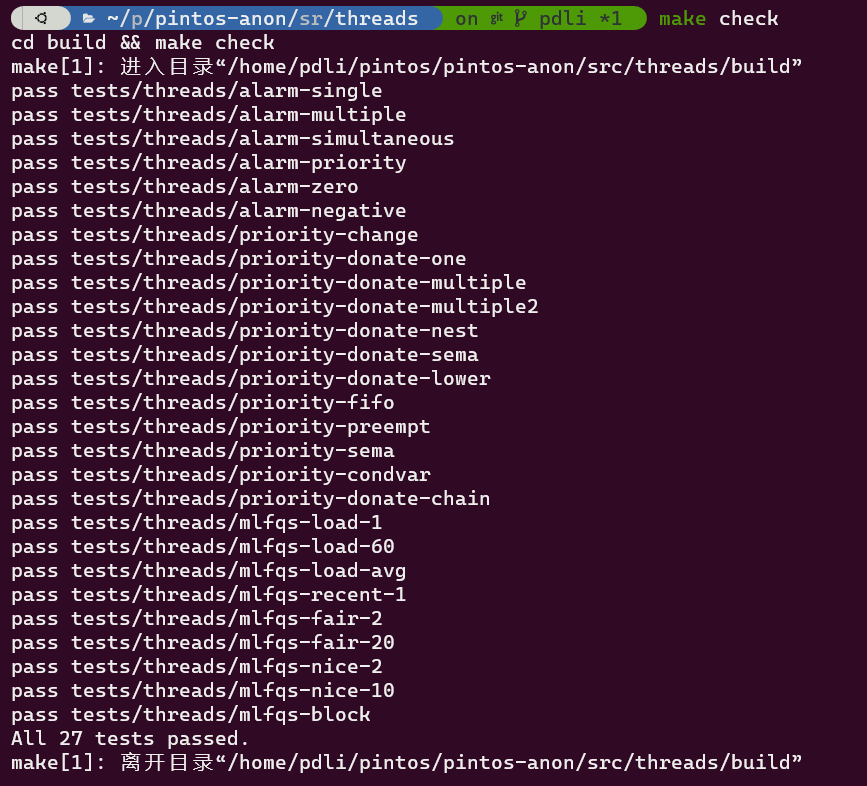
\includegraphics[width=0.65\textwidth]{img/res.png}
  \caption{实验的测试截图}
\end{figure}

在实验中,完成实验的过程如下图所示:

\begin{figure}[H]
  \centering
  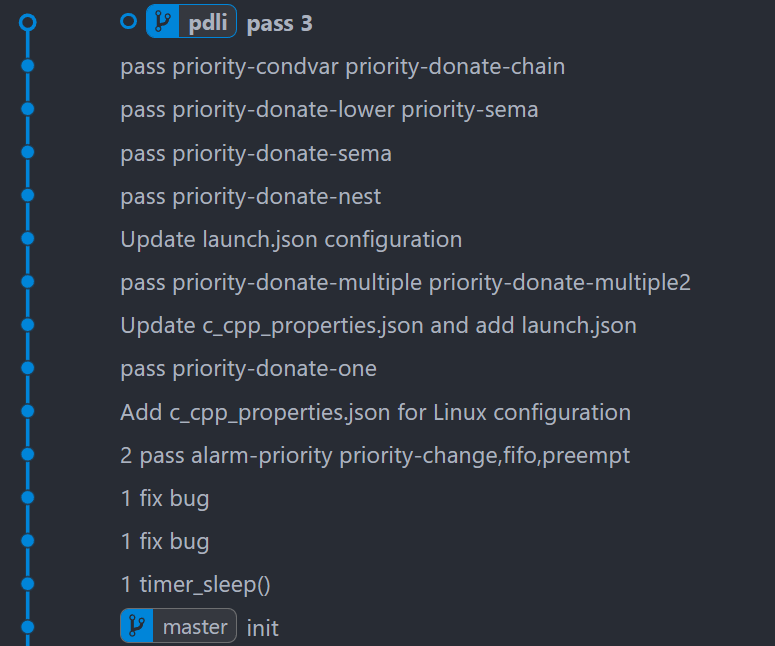
\includegraphics[width=0.8\textwidth]{img/flow.png}
  \caption{实验过程}
\end{figure}

具体实验分析可以参考上文。

\section{实验结果总结}

在本次实验中,我重新实现了 \texttt{timer\_sleep()}函数,使得线程能够在指定的时间内休眠,并且能够在休眠结束后被唤醒。此外,还实现了优先级调度,使得线程能够根据优先级来进行调度。最后,实现了多级反馈队列调度,使得线程能够根据优先级和时间片来进行调度。

通过本次实验,我对操作系统的线程调度有了更深入的了解,同时也对操作系统的实现有了更深的认识。

\normalsize

\section{附录(源代码)}

见 \texttt{source-code-pintos-anon.tar.gz} 或 \texttt{source-code-pintos-anon.zip}。

也可以访问仓库 \url{https://github.com/llipengda/pintos-anon/tree/pdli}。

\normalsize
\end{document}